\documentclass{amsart}
\usepackage{amssymb}
\usepackage{color}
\usepackage{tikz}
\usetikzlibrary{trees,arrows}
\usetikzlibrary{patterns}
\usetikzlibrary{positioning}
\tikzset{mynode/.style={draw,text width=4cm,align=center}
}
\usepackage{tkz-fct,tkz-euclide,tikz-layers}
\tikzset{arrow coord style/.style={dotted, opacity=.8, thin}}
\tikzset{xcoord style/.style={
		font=\footnotesize,text height=1ex,
		inner sep = 0pt,
		outer sep = 0pt,
		text=black}}
\tikzset{ycoord style/.style={
		font=\footnotesize,text height=1ex,
		inner sep = 0pt,
		outer sep = 0pt,
		text=black}}

\begin{document}

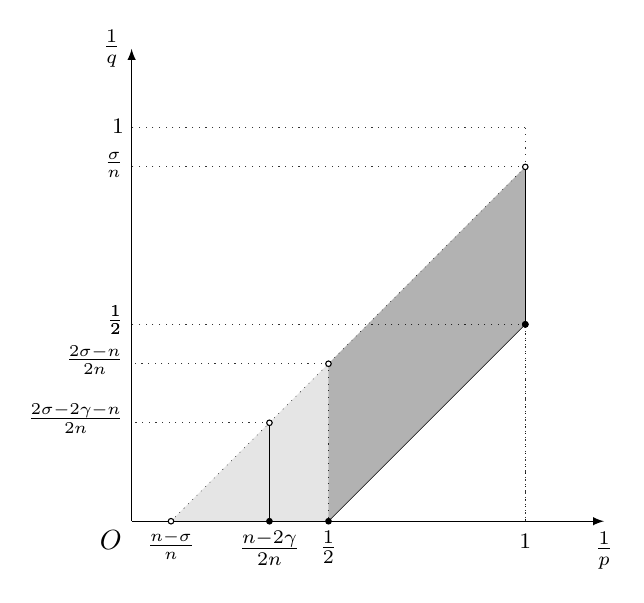
\begin{tikzpicture}[scale=5]
		\tkzInit[xmin=0, xmax=.7, ymin=0, ymax=.70]
		\tkzDrawX[noticks, label=\(\frac{1}{p}\)]
		\tkzDrawY[noticks, label=\( \frac{1}{q}\)]
		\tkzDefPoints{0/0/O}\tkzLabelPoints[below left](O)
		\tkzDefPoints{	0.5/0/A,
			1/.5/B,
			1/1/C,
			0.5/1/D}
		
		\tkzDefPoint(0.5,0){E}
		\tkzDefPoint(1,0.5){F}
		\tkzDefPoint(0.1,0){M}
		\tkzDefPoint(0.35,0){Q}
		\tkzDefPoint(0.35,1){R}
		\tkzDefPoint(0.35,1.1){S}
		\tkzDefPoint(1,0.9){P}
		
		\tkzDefPoint(0.5,0.4){N}
		\tkzDefPointWith[colinear=at M](O,C)\tkzGetPoint{aux}
		
		
		\tkzInterLL(M,N)(Q,R)\tkzGetPoint{I1}
		
		\tkzInterLL(M,aux)(B,C)\tkzGetPoint{M'}
		\tkzInterLL(M,M')(A,D)\tkzGetPoint{I2}		
		
		\tkzPointShowCoord[xlabel=\(1\), ylabel=\(1\), xstyle={below=2mm},ystyle={left=1mm}](C)
		\tkzPointShowCoord[noxdraw,noydraw, ylabel=\(\frac{1}{2}\), xstyle={below=2mm},ystyle={left=1mm}](B)
		
		\tkzPointShowCoord[ylabel=\(\frac{2\sigma-n}{2n}\), xstyle={below=2mm},ystyle={left=1mm}](N)
		
		\tkzPointShowCoord[ylabel=\(\frac{2\sigma-2\gamma-n}{2n}\), xstyle={below=2mm},ystyle={left=1mm}](I1)
		
		\tkzPointShowCoord[ylabel=\(\frac{\sigma}{n}\), xstyle={below=2mm},ystyle={left=1mm}](P)
		
		\tkzPointShowCoord[ylabel=\(\frac{1}{2}\), xstyle={below=2mm},ystyle={left=1mm}](B)
		
		
		\tkzDrawSegment(E,M)
		\tkzDrawSegment[dotted](M,P)
		\tkzDrawSegments(B,P E,F)
		\tkzDrawSegment[black](Q,I1)
		
		\tkzDrawPoints[fill=white](M,B,N,M',I1)
		\tkzDrawPoints[fill=black](A,B,Q)
		\tkzLabelPoint[below](A){\(\frac{1}{2}\)}
		\tkzLabelPoint[below](Q){\(\frac{n-2\gamma}{2n}\)}
		
		\tkzLabelPoint[below,font=\footnotesize](M){\(\frac{n-\sigma}{n}\)}
		
		\begin{scope}[on background layer]
			\tkzFillPolygon[gray!20](M,A,I2)
			\tkzFillPolygon[gray!60](A,B,M',I2)
		\end{scope}
	\end{tikzpicture}

\end{document}